% supposed to be included by another LaTeX document
% as a section
This section describes \qidl\ from the developer's point of view. It explains
general concepts and ideas in section \ref{s_prog_overview}. Section
\ref{s_prog_idlgen} will focus in detail on one of the backbones of
\qidl---the \idlgen\ code generator. The inner workings of the server itself
will be described in section \ref{s_prog_server}.

\qidl\ was designed with some design patterns in mind. Their application is
outlined in section \ref{s_prog_patterns}. These and the overall structure of
\qidl\ make it easy to add new or extend existing functionality. Section
\ref{s_prog_extending} shows the right places to do so.

\subsection{\label{s_prog_overview}General Overview}
The \qidl\ CORBA server runs as as separate thread in the \codine\ master 
executable.
This thread sets up the \master\ object and then blocks and handles
incoming method invocations, while the other thread proceeds as if it ran as
a non-\qidl\ master, i.e. it waits for incoming \codapi\ requests, load reports,
etc. The code that actually executes \codapi\ and \qidl\ requests is exactly the
same. To be precise, each \qidl\ request invokes a local in-process 
\codapi\ request, i.e. one that is not sent over the network.

\subsubsection{Experiences and Concepts}
Several prototypes for evaluating the feasibility of the \qidl\ ideas were
developed and brought up the following results:

\paragraph{Creation of IDL, Header, and Core Implementation Files from Cull
           List Definitions}
  In order to ensure proper maintainability between the main \codine\
  source tree and the \qidl\ sources, the IDL files as well as some C++
  header and implementation files are automatically
  generated from the C header files defining the underlying cull lists. The
  existing cull list definition macros therefore had to be extended to
  provide sufficient information for automatic code generation.
  In addition to the IDL files, cull list definition headers in the standard
  macro format (without the extensions) can be generated. This is useful to
  produce headers for product distribution for use of standard {\tt cod\_api}
  by customers. Lex and yacc are used to scan and parse the C header files.

\paragraph{\qidl\ Integrated in \texttt{cod\_qmaster}}
  Using a separate server daemon for \qidl---as was planned for the first
  approach---requires duplication of all \codine\
  data structures (i.e. cull lists) and thus poses potential problems 
  concerning data integrity. It is therefore wiser to integrate \qidl\ into
  the \texttt{qmaster} executable as a separate thread.
  This offers even faster write access for CORBA clients,
  since their manipulations are directly made upon the master's data.

  The major drawback of this approach is that all read requests cause an
  increase of load in the master executable, thus slowing down performance.
  Even on multiprocessor machines potentially benefiting from
  multithreading, this may affect response times for execution daemons and
  the scheduler.
  In order to limit read access to the master's data,
  an easy-to-use CORBA event interface,
  multiplexed by a standard CORBA event service can propagate data
  changes to event listeners, as described in sections \ref{s_user_events}
  and \ref{s_user_using_qidl_rev}.

\paragraph{Security Problem}
  A standard CORBA compliant ORB offers no way of finding out which user
  sent a request or which host it came from.
  Commercial ORBs usually offer (proprietary) solutions to overcome this 
  problem, but these are usually not available on all desired platforms 
  (especially for LINUX). Furthermore are two different security
  implementations not interoperable, thereby forcing clients to be programmed
  with the same ORB product as the \qidl\ master.

  A glimpse of hope might come from the CORBA security service which is a
  standard CORBA common object service, but as its implementation requires
  modifications in the ORB itself, it is not likely that although two ORBs
  offer this service they will be able to exchange security data. Further
  evaluation will be necessary in this field. The proprietary authentication
  procedure presented in section \ref{s_user_authentication} provides a
  feasible means of passing the desired user and host information to the
  master, but is of course far from what deserves to be called \emph{secure}.

\paragraph{Objects and Lifetime}
  Upon startup, the \qidl\ server will
  create the singleton \master\ object that will always reside on the same
  TCP port (configured by environment variables, command line parameters
  or the like). This is necessary to produce the same IOR each time the 
  server starts.

  In addition to the {\tt Codine::Master} object, the server creates CORBA
  objects that represent the corresponding cull lists from qmaster. That is, all
  objects reside exactly once on one machine in one shared address space. 
  CORBA object references are by definition considered
  persistent. Nonetheless must a client be at any time aware of an object
  reference becoming invalid. This can have either physical reasons (broken
  network connection), logical reasons (a job may have terminated), or
  other reasons (server breakdown). In most of these cases some or all
  object references that a client holds will become invalid. The only
  exception to
  this rule is the {\tt Codine::Master} object, which is always reachable
  under the same address (as long as the server is running, of course).

\subsubsection{Multithreading}
The \qidl\ server consists of two threads: one for the more or less unchanged
\texttt{cod\_qmaster} code for the overall functionality and handling \codapi\
requests (from now on referred to as \emph{master thread}), and one for 
handling \qidl\ CORBA requests (to be called \emph{corba thread}). \qidl\ 
makes use of standard POSIX threads (\textsl{pthreads}) for portability reasons.

Both threads will spend most of the time blocking in a 
\texttt{select()} system call; the master thread waiting for data on the
\texttt{commd} port, the corba thread for requests on the BOA port.
These tasks, as well as marshaling and unmarshaling data, can be done
concurrently. The actual execution of the incoming requests is then mostly
done in the \codine\ kernel code, which is---for historical reasons---not
threadsafe. It is therefore necessary to disallow concurrent execution in the
\codine\ core, which is accomplished by obtaining (and releasing, of course) 
a global mutex variable, \texttt{master\_lock}. The general scheme of
execution is shown in figure \ref{f_prog_locking}, where the two lines
represent the master and corba threads, sequentializing when entering the
\codine\ kernel code.

\begin{figure}
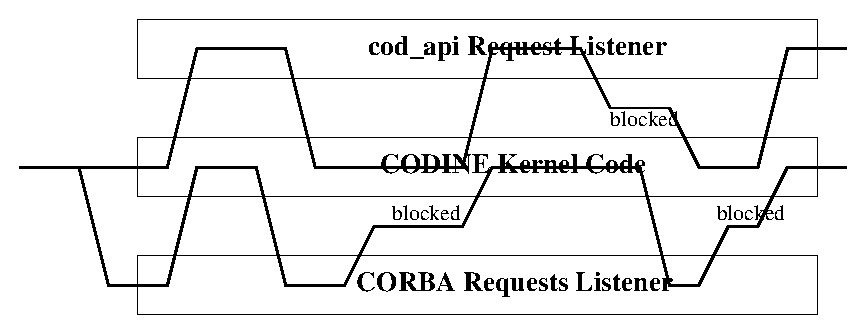
\includegraphics[width=\textwidth]{serverflow.eps}
\caption{\label{f_prog_locking}Concurrent and sequentialized execution of the
master and corba thread.}
\end{figure}

\paragraph{PthreadLock}
To simplify obtaining and releasing locks, a helper class was introduced for
\qidl. In fact, using an automatic class variable provides an elegant means to
release acquired locks in case of an unexpected exception. Consider the
following portion of code, using the standard POSIX C interface for threads:

\begin{Verbatim}[fontsize=\small, frame=single]
void send_event() {
   pthread_mutex_lock(&master_lock);
   
   // invoke CORBA request
   event_channel->push(last_event);
   
   pthread_mutex_unlock(&master_lock);
}
\end{Verbatim}

This code usually works fine. But invoking a CORBA request can always yield
an exception; be it a NIL object reference, a communication failure, or
whatever. In
this case, the \texttt{pthread\_mutex\_unlock()} command is never executed
and the lock never released. Instead of enclosing the critical sections in
explicit \texttt{try\dots catch} statements, a simple local variable solves
this problem in a more elegant way:

\begin{Verbatim}[fontsize=\small, frame=single]
void send_event() {
   PthreadLock lock(&master_lock); // this locks the mutex in the c'tor
   
   // invoke CORBA request
   event_channel->push(last_event);

   // leaving the block unlocks the mutex in the variable's d'tor
}
\end{Verbatim}

The local variable \texttt{lock} obtains the mutex variable when it is
created. Since C++ guarantees that all local objects' destructors are called
when they get out of scope, the lock is released no matter how the function
terminates.

Another advantage of using a class shows up when one function in a thread
(which has successfully acquired the lock) makes a call to another function,
which in turn tries to obtain the lock again. According to the pthreads
standard, this results in undefined behavior---usually a dead-lock. To solve
this problem, the \texttt{PthreadLock} class maintains an internal per-thread
reference count of each mutex variable. If one thread tries to acquire a lock
of a mutex variable more than once, it is not actually locked, but its
reference counter is increased---and decreased in the destructor, respectively.
If the reference count reaches zero, the mutex variable is actually
unlocked. \texttt{PthreadLock}'s interface is as follows:

\begin{Verbatim}[fontsize=\small, frame=single]
class PthreadLock {
   public:
      PthreadLock(pthread_mutex_t* m);
      ~PthreadLock();

      // avoid calling these unless you know what you're doing
      void     lock();
      void     unlock();
      
      static bool initialize();
   
   private:
      static bool init;

      static pthread_mutex_t lock;

      // stores a map<pthread_mutex_t*, unsigned int>
      static pthread_key_t key; 
      // the PthreadLock object's mutex
      pthread_mutex_t*     mutex;
      
      static void destroy(void* state)
         {delete (map<pthread_mutex_t*, unsigned int>*)state;}
};
\end{Verbatim}

\texttt{PthreadLock::initialize()} must be called before the first usage of
the class. It creates the pthread key variable, using the static
\texttt{PthreadLock::\-destroy()} function to cleanup memory. The per-thread
reference count is stored in a \texttt{map<pthread\_mutex\_t*, unsigned int>},
which associates the reference counter with its mutex. To further simplify
usage, the following macro is defined:

\begin{Verbatim}[fontsize=\small, frame=single]
#define AUTO_LOCK_MASTER PthreadLock lock(&master_lock);
\end{Verbatim}

\subsubsection{Source Files and their Dependencies}
The \qidl\ source directory is relatively small, whereas the ready compiled
executable can be several megabytes in size. That's because a large part of
the \qidl\ server code is automatically generated out of the api header
files. This makes the overall compilation process pretty complicated---and
thus the makefile, too.

\qidl\ is built around \emph{objects}, and that's why the makefile defines a
variable \texttt{OBJECTS} as:
\begin{Verbatim}[fontsize=\small, frame=single]
OBJECTS    = Queue. \
             ComplexEntry. \
             Complex. \
             Job. \
             PathName. \
             MailRecipient. \
             Variable. \
             ConfigEntry. \
             Configuration. \
             Range. \
             Calendar. \
             String. \
             Checkpoint. \
             QSCommand. \
             QueueingSystem. \
             ExecHost. \
             HostLoad. \
             LoadScaling. \
             PathAlias. \
             ParallelEnvironment. \
             Request. \
             SchedConf. \
             SubordinateQueue. \
             Usage. \
             UserEntry. \
             UserProject. \
             UserSet.
\end{Verbatim}
This contains the names of all interfaces and structs and can easily be
extended. A shell script called \texttt{make\_obj\_rules.sh}, which is
invoked by \texttt{make depend}, creates appropriate rules for these objects
to create their IDL, header, and implementation files. The overall dependencies
can be seen from figure \ref{f_prog_dependencies}.

\begin{figure}[b!]
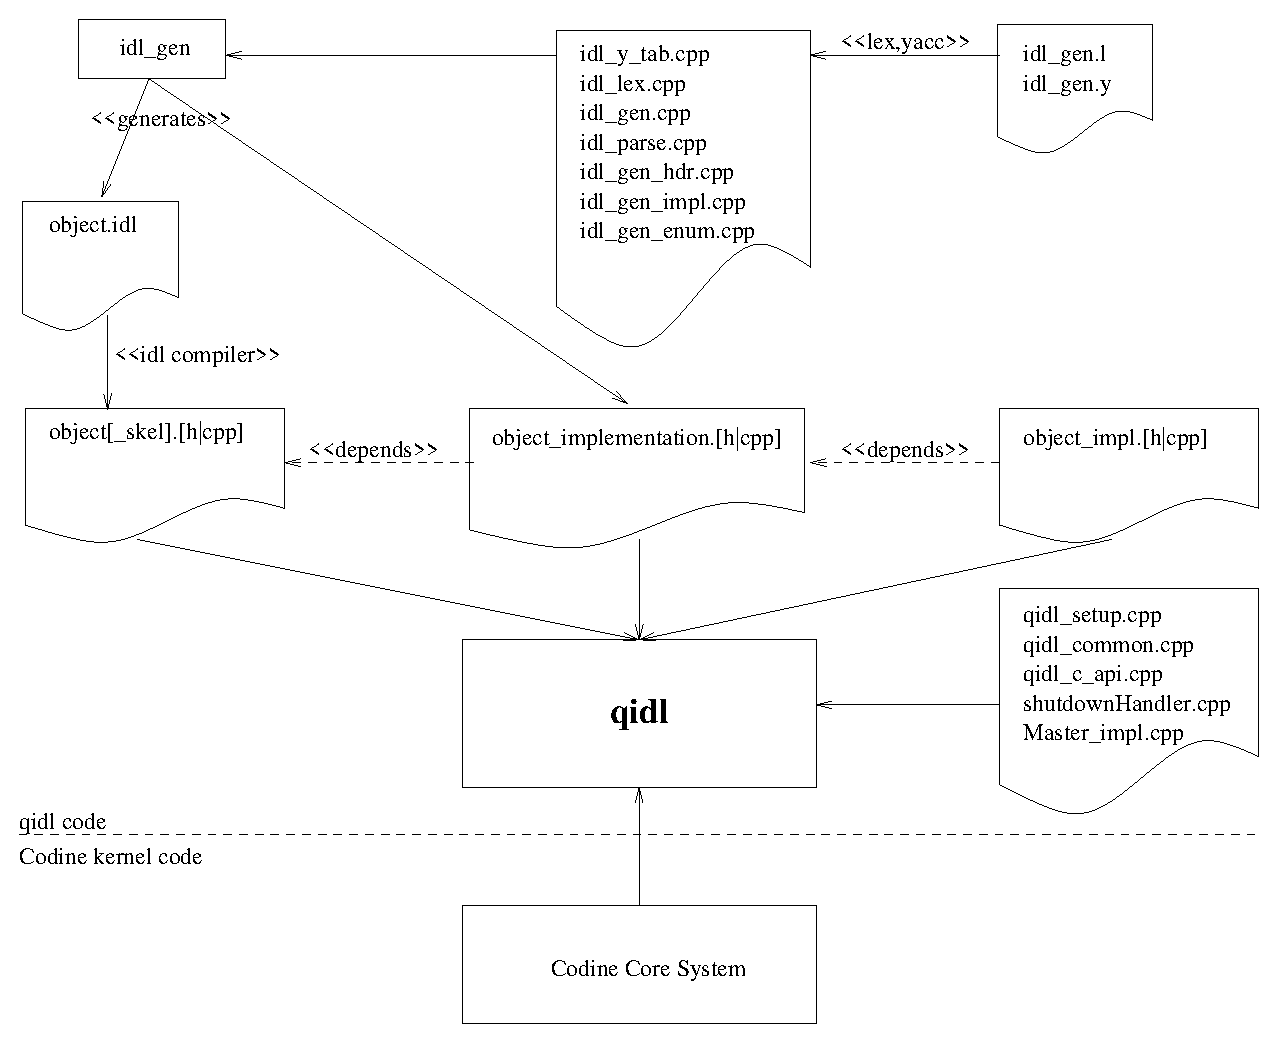
\includegraphics[width=\textwidth]{filedep.eps}
\caption{\label{f_prog_dependencies}The dependencies of the \qidl\ files.}
\end{figure}

Although some auxiliary files and header file dependencies have been
omitted, the diagram looks pretty complex, especially considering the
dependencies between \texttt{object\_skel, \_implementation,} and
\texttt{\_impl}, where the order of compilation and generation is extremely
important.

\subsection{\label{s_prog_idlgen}The Code Generator}
{\tt idl\_gen} is the utility to translate the cull list definitions from the
header files into 
\begin{itemize}
\item OMG CORBA IDL files
\item class headers for object implementation
\item partial object implementation
\item a file containing constants for attribute names.
\end{itemize}
It is also used to create headers for the
distribution release of {\tt cod\_api} cull headers. These headers will only
contain the standard cull list macros without any of the extensions
introduced in the following section. 

The command line syntax is as follows:

\begin{Verbatim}[fontsize=\small, frame=single]
idl_gen [-noidl] [-nohdr] [-noimpl] [-noelemcodes] [-nodisthdr] 
        input-files
        [-of files] [-oo objects]
\end{Verbatim}

where:
\begin{description}
\item[-noidl]      suppresses output of IDL files.
\item[-nohdr]      suppresses output of \texttt{\_implementation.h} files.
\item[-noimpl]     suppresses output of \texttt{\_implementation.cpp} files.
\item[-noelemcodes]suppresses output of \texttt{elem\_codes.idl} file.
\item[-nodisthdr]  suppresses output of .h.dist files.
\item[-of]         produces output only for objects that are defined in the
             following list of files.
\item[-oo]         produces output only for the given objects.
\item[input-files] is a list of files that contain cull list definitions.
\item[files]       is a list of files for whose objects output will be produced.
\item[objects]     is a list of object names for which output will be produced.
\end{description}

If -of or -oo are not given, \texttt{idl\_gen} produces output for all 
files or objects.  If specified, \emph{both} -oo and -of requirements must 
be met for an object.  That is, no output will be produced for the 
following command line:

\begin{Verbatim}[fontsize=\small, frame=single]
idl_gen cod_calendarL.h cod_queue.h -of cod_calendar.h -oo Queue
\end{Verbatim}

The order of the -oo and -of switches is not important as long as they occur 
after the input file list. It is also valid to have multiple -of and -oo
switches in one command line and to specify the same file or object more than 
once, or even to specify files that don't exist.
-of and -oo have no effect on distribution header output: .h.dist files are 
always produced, unless -nodisthdr is specified.

\texttt{idl\_gen} will create several files as shown in figure
\ref{f_prog_dependencies} on page \pageref{f_prog_dependencies}.
Since cull lists usually reference each other, the created files
will correctly \texttt{\#include} each other as appropriate. The program aborts
with an error when a reference could not be resolved successfully.

\subsubsection{Cull Macro Extensions}
As mentioned previously, the IDL and partial object implementation
files will be automatically 
generated from the C header files defining the cull lists. \idlgen\ 
(generated with the aid of lex and yacc) parses the desired header files 
and produces proper output files which do not have to be modified anymore and 
can thus be integrated smoothly in the build process via makefiles.

It is obvious that the previously existing macros for cull definition are by
far not sufficient for this purpose. The following paragraphs describe the 
extensions that have been necessary to accomplish this task.

It should be noted that these extensions are only required for the build
process of \qidl. In order to avoid unnecessary complexity of the header
files in the distribution and possible confusion of customers, it is highly
recommended that these extension only be used in the development tree of
\codine. \texttt{idl\_gen} offers a way to
produce standard cull list definition files out of the extended files.

\paragraph{List Definition}
\subparagraph{MACRO TYPE}
\begin{verbatim}
   LISTDEF
\end{verbatim}

\subparagraph{SYNTAX}
\begin{verbatim}
   ILISTDEF( type, name )
   SLISTDEF( type, name )
   XLISTDEF( type , name )
   LISTDEF( type )
\end{verbatim}

\subparagraph*{DESCRIPTION}
   This macro begins a list definition. The I and S forms will produce
   IDL output, where the name of the IDL interface is {\it name}. {\it Type}
   specifies the cull list type (e.g. JB\_Type). It is used by \qidl\
   for referencing objects.
      
   The ILISTDEF variant will produce a CORBA interface, whereas 
   SLISTDEF will create a struct. Use ILISTs for global
   objects and SLISTs for others. SLISTs need an additional parameter that
   specifies the name of the master list, where the objects are stored, e.g.
   MASTER\_QUEUE\_LIST for queues.
   
   The third form will not produce IDL output and should be used
   to indicate that no IDL interface will be generated.
   
   The last form is the standard list definition used by \codine. It will
   not produce IDL output and is considered obsolete but still supported
   for backward compatibility.

\paragraph{Standard List Entry}
\subparagraph{MACRO TYPE}
\begin{verbatim}
   COD_ELEM
\end{verbatim}

\subparagraph{SYNTAX}
\begin{verbatim}
   COD_ELEM( name )
   COD_RELEM( name )
   COD_IELEM( name )
   COD_IRELEM( name )
   COD_XELEM( name )
\end{verbatim}
   
   where ELEM is one of [ INT $|$ STRING $|$ FLOAT $|$ DOUBLE $|$ CHAR 
   $|$ LONG $|$ ULONG ]

\subparagraph{DESCRIPTION}
   These macros are used to define a list element for a cull list and/or a
   data member for an IDL interface/struct. The R variants produce a
   readonly attribute in IDL interfaces. In IDL structs and cull lists this
   shows no effect. Note that elements are not mapped to IDL attributes
   because of the context and raises clauses, but to get\_ and set\_ functions.

   The I variants produce data members only in IDL interfaces/structs but
   do not appear in cull lists. XELEMs are their counterpart: no IDL
   output, but standard cull meaning.

\paragraph{Object References And Aggregation}
\subparagraph{MACRO TYPE}
\begin{verbatim}
   COD_LIST, COD_OBJECT
\end{verbatim}

\subparagraph{SYNTAX}
\begin{verbatim}
   COD_TLIST( name, type )
   COD_ILIST( name, type )
   COD_RLIST( name, type )
   COD_IRLIST( name, type )
   COD_XLIST( name , type )
   COD_OBJECT( name, type )
   COD_IOBJECT( name, type )
   COD_ROBJECT( name, type )
   COD_IROBJECT( name, type )
   COD_XOBJECT( name, type )
   COD_LIST( name )
\end{verbatim}

\subparagraph{DESCRIPTION}
   These macros are used to define references to objects and aggregation of
   structs. All of them except ILIST and IOBJECT will result in a standard
   cull list entry as expected for LIST. The I variants will produce IDL output
   only. {\it name} is the name of the element that will appear in the cull list
   and in the IDL interface/struct (without prefix for the latter), and
   {\it type} is the type of interface/struct referenced and must be a type 
   that is defined with a LISTDEF macro. If the given type is unknown, no IDL 
   output will be generated for this entry.

   TLIST, ILIST, RLIST, and IRLIST  are used for sequences of the given type,
   whereas OBJECT references/contains exactly one instance of the given type.
   The R variants will produce a readonly attribute in objects and has no
   special meaning for IDL structs or cull lists.

   XLIST will not produce IDL output, but does appear in cull lists. The
   plain LIST variant without a type argument should be considered obsolete
   and is supposed to be replaced by XLISTs. This also serves documentation
   purposes.

   LIST is the old LIST macro with one parameter as
   used for cull lists before \qidl. It is considered obsolete and should
   not be used anymore. No IDL code is generated for this.

   TLIST should have actually be named LIST, but due to backwards
   compatibility to the old LIST macro another name had to be chosen.

\paragraph{Miscellaneous}
\subparagraph{MACRO TYPE}
\begin{verbatim}
   LISTEND
\end{verbatim}

\subparagraph{SYNTAX}
\begin{verbatim}
   LISTEND
\end{verbatim}

\subparagraph{DESCRIPTION}
   This macro ends a list definition and is not altered from the standard
   cull format.


\subparagraph{MACRO TYPE}
\begin{verbatim}
   IDL
\end{verbatim}

\subparagraph{SYNTAX}
\begin{verbatim}
   /*IDL
      idl_code
   XIDL*/
\end{verbatim}

\subparagraph{DESCRIPTION}
   Anything placed between and IDL/XIDL pair will be copied as is into the
   resulting IDL file. Use these "macros" to add special methods to an IDL
   interface.

   Note that the IDL section is a standard C multiline comment and will
   thus be ignored for cull lists. Be sure not to have other /* */ pairs
   between IDL and XIDL that may confuse the compiler. Only use // for
   IDL comments.

%\paragraph{Example}
%\begin{verbatim}
%CLISTDEF( JB_Type, Job )
%   COD_RULONG( JB_job_number )
%   COD_STRING( JB_script_file )
%   COD_XULONG( JB_uid )
%   COD_LIST( JB_stdout_path_list, PN_Type )
%   COD_IROBJECT( JB_queue, QU_Type )
%   COD_XLIST( JB_hard_queue_list, QR_Type )
%   COD_ILIST( JB_hard_queue_list, QU_Type )
%   IDL
%      void suspend();  // suspends this job
%   XIDL
%LISTEND
%
%SLISTDEF( PN_Type, PathName )
%   STRING( PN_path )
%   STRING( PN_host )
%LISTEND
%\end{verbatim}
%
%This excerpt from a C header file produces the following IDL code:
%
%\begin{verbatim}
%module Codine {
%   interface Job : Obj {
%      readonly attribute ulong job_number;
%               attribute string script_file;
%               attribute PathNameSeq stdout_path_list;
%      readonly attribute Queue queue;
%               attribute QueueSeq hard_queue_list;
%      void suspend();  // suspends this job
%   };
%
%   struct PathName {
%      string path;
%      string host;
%   };
%};
%\end{verbatim}

\subsubsection{Lex and Yacc}
\texttt{lex} and \texttt{yacc} will be used to produce a parser for cull
header files. This parser understands the keywords defined in the previous
section, "Cull Macro Extensions", and ignores everything else. The main
program (\texttt{idl\_gen.cpp}) will call this parser on all input files,
thus generating meta information stored in the data structures defined in
\texttt{idl\_repository.h}. It then calls several functions
that analyze the meta data and generate the desired
output. The distribution headers (if desired) are generated on the fly when
parsing the input files.

In the parsing process itself, the meta data structures are filled. These are
simple structs containing information for each parsed cull list and its
elements. This includes mainly names and data type information. They make
extensive use of the C++ Standard Template Library (STL) and can be accessed
easily. The actual code generator functions iterate over the meta data and
produce the desired output.

\subsubsection[From Cull to IDL]{\label{s_prog_skeleton}
                             From Cull to IDL---Or: The Server Skeleton}
The most important files generated by \idlgen\ are the OMG CORBA IDL files,
describing the public interfaces of the \codine\ objects. All interfaces are
embedded in a namespace \texttt{Codine} and derived from the base interface
\texttt{Codine::Obj}. There is not very much to do for the IDL code
generator. Apart from writing the file header and footer, it creates a
\texttt{get\_} and (if not read-only) a \texttt{set\_} function for each
element in the list's meta data structure, always appending the
\texttt{raises} and \texttt{context} clauses. The last task is to append the
inlined \texttt{/*IDL\dots XIDL*/} code from the cull list definitions.

\subsubsection[Basic Implementation]{\label{s_prog_flesh}
                     Basic Implementation---Or: The Flesh around the Bones}
Creating the implementation header and source files is by far more complicated
than creating the IDL files. That is to say that the \emph{creation}
itself is not difficult---it only consists of some stream operations just like 
the ones for the IDL files. The intelligence lies in the \emph{contents} of
the produced files, which provide code that otherwise would have to be written 
by hand in an ever-reoccuring pattern. Now let's take a look at the details of 
the files.

\paragraph{Implementation Header}
The \texttt{\_implementation.h} file contains a complete class declaration
for an IDL interface implementation (conforming to ORBacus' BOA
implementation). It is therefore derived \texttt{public virtual} from the
corresponding \texttt{\_skel} class created by the IDL compiler from the IDL
file. Apart from constructor and destructor, the class declares prototypes of
all methods defined in the object's interface. Functions that involve
references to other objects (not structs!) are declared pure virtual, i.e.
they have to be implemented by yet another subclass, as described in section
\ref{s_prog_server_objects}.

There are some other class members as well. To be precise, these are:
\begin{Verbatim}[fontsize=\small, frame=single]
class Some_implementation : virtual public Some_skel {
   // ...

   protected:
      CORBA_String_var          key;
      lListElem*                self;
      lListElem*                newSelf;
      virtual lListElem*        getSelf() = 0;
      CORBA_ORB_var             orb;
      time_t                    creation;
      cod_ulong                 lastEvent;
   friend class Codine_Master_impl;
};
\end{Verbatim}
\begin{description}
\item[key] is the unique object name. For jobs this is not a string but an
integer value.
\item[self] is a pointer to the object's underlying cull list.
\item[newself] is used in conjunction with events.
\item[getSelf()] returns a pointer to the object's underlying cull list. This
function must be implemented by a subclass and usually makes an 
\texttt{lFindFirst()} call.
\item[orb] is the ORB's object reference.
\item[creation] is the object's creation time. It is non-zero for newly
created objects (i.e. those visible only to their creator).
\item[lastEvent] is the integer value of the last event associated with this
object.
\end{description}

\paragraph{Implementation File}
The \texttt{\_implementation.cpp} file is more interesting. It mainly
contains the implementations of all \texttt{get\_} and \texttt{set\_}
functions except the ones that concern references to other \codine\ objects.
The first lines of each of these functions are exactly identical and look
like this (taken from \texttt{Codine\_Queue\_implementation::\-get\_qhostname}):

\begin{Verbatim}[fontsize=\small, frame=single]
cod_string Codine_Queue_implementation::get_qhostname(
                                          CORBA_Context* ctx) {
   QENTER("Queue::get_qhostname");
   AUTO_LOCK_MASTER;
   qidl_authenticate(ctx);
   if(!getSelf()) {
      orb->disconnect(this);
      CORBA_release(this);
      throw Codine_ObjDestroyed();
   }

   // ...
}
\end{Verbatim}

These commands
\begin{enumerate}
\item print debug/trace output,
\item acquire the global mutex variable,
\item validate the delivered context variable (throws an exception in case
      of an error),
\item retrieve the object's underlying cull list, and if this is not
      successful
   \begin{enumerate}
   \item disconnects the CORBA object from the ORB, and
   \item throws an appropriate exception.
   \end{enumerate}
\end{enumerate}

This block is followed by some attribute and data type specific lines, like
these for a string type:

\begin{Verbatim}[fontsize=\small, frame=single]
cod_string Codine_Queue_implementation::get_qhostname(
                                       CORBA_Context* ctx) {
   // ...

   char* temp = lGetString(self, QU_qhostname);
   cod_string foo = CORBA_string_dup(temp?temp:"");
   return foo;
}
\end{Verbatim}

Comparing this to a \texttt{cod\_ulong} typed attribute reveals a common
pattern:

\begin{Verbatim}[fontsize=\small, frame=single]
cod_ulong Codine_Queue_implementation::get_seq_no(CORBA_Context* ctx) {
   // ...

   cod_ulong foo = lGetUlong(self, QU_seq_no);
   return foo;
}
\end{Verbatim}

\begin{enumerate}
\item Retrieve the attribute's value from the cull,
\item make a copy of the value considering a NULL pointer (strings only), and
\item return the value.
\end{enumerate}

Very easy, isn't it? If this code wasn't generated automatically, someone
would have to hand-write code like this for hundreds of attributes---cearly
unsatisfying. What about attributes with structs as their data type? Here's
the code:

\begin{Verbatim}[fontsize=\small, frame=single]
Codine_ComplexEntrySeq* 
      Codine_Queue_implementation::get_consumable_config_list(
      CORBA_Context* ctx) {
   // ...

   lList* lp = lGetList(self, QU_consumable_config_list);
   Codine_ComplexEntrySeq* foo = cull2ComplexEntrySeq(lp);
   return foo;
}
\end{Verbatim}

\label{p_converters}
The only difference is the call to the \texttt{cull2ComplexEntrySeq()}
function. As its name implies, it converts a cull list to a
\texttt{Codine::ComplexEntrySeq}. There are many functions like
\texttt{cull2XXXSeq()} and \texttt{XXXSeq2cull()} which convert CORBA
sequence types to and from their corresponding cull list type. In spite of
all automation, these functions have to be written by hand, but they are
really easy and need not be mentioned here.

The \texttt{set\_} functions are somewhat more interesting. Each of these
requests is translated into a local \codapi\ request because
\begin{itemize}
\item \codapi\ is a tested and reliable interface,
\item it eliminates the danger of data inconsistency, since data is manipulated
      by the same portion of code for both \codapi\ and \qidl\ requests,
\item user access rights need not be checked explicitly for a \qidl\ request,
\item proper event handling is guaranteed for both \qidl\ event clients and 
      the \codine\ scheduler.
\end{itemize}
So the code looks as follows:

\begin{Verbatim}[fontsize=\small, frame=single]
cod_ulong Codine_Queue_implementation::set_qhostname(const char* val,
                                                  CORBA_Context* ctx) {
   // usual function header omitted...

   if(creation != 0) {
      lSetString(self, QU_qhostname, (char*)val);
      return 0;
   }

   lListPtr      lp;
   lListPtr     alp;
   lListElem*   lep;
   lEnumeration* what;

   lp = lCreateList("My qhostname list", QU_Type);
   lAppendElem(lp, (lep = lCopyElem(self)));
   lSetString(lep, QU_qhostname, (char*)val);
   what = lWhat("%T(%I %I)", QU_Type, QU_qname, QU_qhostname);
   alp = cod_api(COD_QUEUE_LIST, COD_API_MOD, &lp, NULL, what);
   lFreeWhat(what);
   throwErrors(alp);
   return lastEvent;
}
\end{Verbatim}

The function first checks if the object's creation time is non-zero, i.e. if
the object is still "under construction" by a user and not yet publicly
visible. In this case, the modification of the attribute can be done in the
local \texttt{self} cull list. Since no event will be generated for this,
the function returns 0 as the event number.

The other case, i.e. modifying a global object requires a bit more work.
\codapi\ programmers might find the code familiar. All there is to do is
\begin{enumerate}
\item setting up a cull list,
\item appending a copy of the object's cull,
\item modifying the appropriate value,
\item setting up an \texttt{lEnumeration} to define the scope of the request,
\item issue the \codapi\ call, 
\item cleaning up the data structures, and
\item returning the event number to the caller.
\end{enumerate}

There are two features worth mentioning here. The first one is the \codapi\
call itself. It looks like a standard \codapi\ invocation, one like any other
\codapi\ could have done, too. The only difference is that the function's
implementation recognizes that it was called from \emph{inside} the master
executable and thus does not send the request over the network, but simply
passes it on directly to the receiver function.

The second feature concerns the 6th item, cleaning up. The attentive reader
may have noticed that the cull lists are not freed with a call to
\texttt{lFreeList()}. That is because the standard \texttt{lList*}s have been
replaced by a \texttt{lListPtr} class, which cares for automatic memory
management and defines some conversion functions for convenient usage in the
standard \codapi\ context.

Like the \texttt{PthreadLock} facility, this feature was driven by 
Elegan$C^{++}$e concerning exception handling. Notice the line
\texttt{throwErrors(alp);} in the code above. This is a custom function that
converts the answer list returned by a \codapi\ call into a
\texttt{Codine::Error} exception---if an error occured, that is. If
everything went well, nothing happens and the function returns happily. In
both cases, the lists' memory has to be freed, which would require ugly
\texttt{try\dots catch} clauses, hadn't these \texttt{lListPtr} classes been
used.

The code for setting attributes with fundamental data types other than
string is very similar to the one shown above. Even handling \texttt{struct}
types isn't really more work:

\begin{Verbatim}[fontsize=\small, frame=single]
cod_ulong Codine_Queue_implementation::set_migr_load_thresholds(
               const Codine_ComplexEntrySeq& val, 
               CORBA_Context* ctx) {
   // ...

   lp = lCreateList("My migr_load_thresholds list", QU_Type);
   lAppendElem(lp, (lep = lCopyElem(self)));
   lSetList(lep, QU_migr_load_thresholds,
               ComplexEntrySeq2cull((Codine_ComplexEntrySeq&)val));
   what = lWhat("%T(%I %I)", QU_Type, QU_qname, QU_migr_load_thresholds);
   alp = cod_api(COD_QUEUE_LIST, COD_API_MOD, &lp, NULL, what);
   lFreeWhat(what);
   throwErrors(alp);
   return lastEvent;
}
\end{Verbatim}

The only real difference is the call to \texttt{ComplexEntrySeq2cull()},
which does exactly that. See page \pageref{p_converters} earlier in this
section for more information.

The last major content of the \texttt{\_implementation.cpp} file is the
implementation of get \texttt{get\_} and \texttt{set\_content()} functions.
These are usually lengthy methods, since they must assemble or disassemble a
\texttt{Codine::contentSeq} that represents the complete object state.
\texttt{get\_content()} is significantly easier to write than
\texttt{set\_content()}, because the latter requires some tricky, admittedly 
hard to understand code. But let's start with the first of the two,
\texttt{get\_content()}:

\begin{Verbatim}[fontsize=\small, frame=single]
Codine_contentSeq* Codine_Queue_implementation::get_content(
                                                CORBA_Context* ctx) {
   // usual function header ...

   // build content sequence
   Codine_contentSeq* cs = new Codine_contentSeq;
   char* dummy;

   cs->length(24);         // i.e. the number of attributes

   // qname
   cs->operator[](0).elem = Codine_QU_qname;
   cs->operator[](0).value <<= CORBA_string_dup(
                     (dummy = lGetString(self, QU_qname))?dummy:"");
   // seq_no
   cs->operator[](4).elem = Codine_QU_seq_no;
   cs->operator[](4).value <<= (cod_ulong)lGetUlong(self, QU_seq_no);
   // load_thresholds
   cs->operator[](5).elem = Codine_QU_load_thresholds;
   cs->operator[](5).value <<= get_load_thresholds(
                   Codine_Master_impl::instance()->getMasterContext());
   // complex_list
   cs->operator[](22).elem = Codine_QU_complex_list;
   cs->operator[](22).value <<= get_complex_list(
                   Codine_Master_impl::instance()->getMasterContext());
   // other attributes follow...
   
   return cs;
}
}\end{Verbatim}

This code is pretty straightforward. The function simply sets up a
\texttt{content\-Seq} and fills its entries with reasonable name/value
pairs. For \texttt{struct} and reference type attributes, it makes use of its
own \texttt{get\_} functions described earlier in this subsection. This is
possible, since the \texttt{value} of the \texttt{Codine::contentSeq} is of
type \texttt{CORBA::Any}, and with the \texttt{<<=} operator virtually any
user defined type can be assigned to the \texttt{value} variable.

For the \texttt{set\_content()} method, the code is not quite that simple:

\begin{Verbatim}[fontsize=\small, frame=single]
cod_ulong Codine_Queue_implementation::set_content(
               const Codine_contentSeq& cs, CORBA_Context* ctx) {
   // usual function header...

   // intermediate variables, not all may be used
   Codine_ComplexEntrySeq* ComplexEntry_val;
   Codine_ComplexSeq* Complex_val;
   cod_float Float_val;
   cod_double Double_val;
   cod_ulong Ulong_val;
   cod_long Long_val;
   cod_char Char_val;
   cod_int Int_val;
   cod_string String_val;
   lList* List_val;
   lListPtr lp = lCreateList("set content", QU_Type);
   lListElem* lep = lCreateElem(QU_Type);
   lAppendElem(lp, lep);

   // now pretend we're CORBA-only
   time_t old_creation = creation;
   creation = 1;
   lListElem* oldSelf = self;
   self = lep;
   
   // check the sequence
   for(CORBA_ULong i=0; i<cs.length(); i++) {
      switch(cs[i].elem) {
      case QU_qname:
         cs[i].value >>= String_val;
         lSetString(lep, QU_qname, String_val);
         break;
      case QU_seq_no:
         cs[i].value >>= Ulong_val;
         lSetUlong(lep, QU_seq_no, Ulong_val);
         break;
      case QU_load_thresholds:
         cs[i].value >>= ComplexEntry_val;
         List_val = ComplexEntrySeq2cull(*ComplexEntry_val);
         lSetList(lep, QU_load_thresholds, List_val);
         break;
      case QU_complex_list:
         cs[i].value >>= Complex_val;
         set_complex_list(*Complex_val, 
                  Codine_Master_impl::instance()->getMasterContext());
         break;
   }

   // don't forget to set back
   creation = old_creation;
   self = oldSelf;

   // now set the state
   if(creation) {
      lFreeElem(self);
      self = lCopyElem(lep);
   }
   else {
      lListPtr alp;
      lEnumeration* what = lWhat("%T(ALL)", QU_Type);
      alp = cod_api(COD_QUEUE_LIST, COD_API_MOD, &lp, NULL, what);
      lFreeWhat(what);
      throwErrors(alp);
   }

   return lastEvent;
}
}\end{Verbatim}

Have a look at the \texttt{for} loop in the middle of the code, first. It
iterates through the given sequence and checks which elements are supplied in
it. Note that this sequence need not be complete and can come in any order,
so the \texttt{for} and \texttt{switch} statements are necessary.
First of all, the content of the \texttt{Any} value has to be extracted into
local variables, declared at the top of the code. The \texttt{>>=} operator
ensures type safety here. 

For simple and \texttt{struct} types, simply setting the extracted value
(converting it to a cull list for \texttt{struct}s) in the soon-to-be new
object state cull is all there is to do. Object reference types (such as the
\texttt{complex\_list} above) make things more complicated. You can see, that
again, it's only one line of code, \texttt{set\_complex\_list(\dots)}. But to
make this work, several preconditions have to be met.

First of all, the object must pretend that it is \emph{CORBA-only}, i.e. not
publicly visible to all \codine\ users, since the latter would force the
\texttt{getSelf()} method, called by the \texttt{set\_complex\_list()} method
to get the current object state from the \codine\ master object store, thus
overriding any local changes made up to this point. Then it has to
temporarily set the \texttt{self} variable to the above mentioned soon-to-be
new object state cull. This makes \texttt{getSelf()} return this (actually
local) variable and \texttt{set\_complex\_list()} alter the correct value.
This mechanism would work for all attributes, too, and not only for object
reference types. But the simplicity of inline implementation and the
otherwise necessary function call overhead (including the usual function
header, remember) makes the current implementation much faster.

After the cull list has been set up correctly for all delivered attributes,
the changed variables \texttt{creation} and \texttt{self} are reset to their
original values. Then the new object state is either set locally, or set as
the global state with a \codapi\ call. This creates an event, and its counter
is returned from the function.

The \idlgen\ code generator provides a broad basis that the \qidl\ server can
be built upon. Especially the two \texttt{\_implementation.[h$|$cpp]} files
relief the programmer of some monotonous and error-prone copy\&paste work.
But still some parts have to be implemented by hand, as described in the
following section.

\subsection[The Server]{\label{s_prog_server}The Server---Or: Adding Skin 
                                             and Brain}
Think of the \qidl\ servers as a human (or, for that matter, any mammal)
body: There's a skeleton, forming the overall shape. This is
represented by the IDL interfaces, described in section
\ref{s_prog_skeleton}. The body's muscles and flesh strengthen its structure
and provide the means to accomplish some simple tasks---the server's base
implementation as presented in section \ref{s_prog_flesh}. To round off the
body's overall appearance and to bring life and meaning to it, it needs skin
(additional and convenience functions) and---most important---a brain, i.e.
the \master\ object. It's like having Frankenstein's monster assembled
automatically, just adding the interesting parts by hand. The following
subsections show how this is done for the \qidl\ "monster".

\subsubsection{The Master}
Recall from section \ref{s_userdoc} that the \master\ object is the entry point
for a \qidl\ client into the \codine\ system. From here, all other objects
can be accessed and new ones created. Event handling and other functions are
offered, too. Let's take a look at the master's header file. The remainder of
this subsection will pinpoint some important and interesting features of its
implementation and frequently refers to some lines is this header file. You
may want to skip back to this page and have a closer look at the referenced
class members. You may also find a comparison with the master's IDL file 
valuable in understanding the overall concept.

\begin{Verbatim}[frame=lines, numbers=left, fontsize=\small, framerule=1mm]
class Codine_Master_impl : virtual public OBEventHandler, 
                         virtual public Codine_Master_skel, 
                         virtual public CosEventComm_PushSupplier_skel {
   private:
      static Codine_Master_impl* master;

   protected:
      Codine_Master_impl(CORBA_ORB_ptr o, CORBA_BOA_ptr b);
      virtual ~Codine_Master_impl();

      // OBEventHandler stuff, sends event when notified
      virtual void handleEvent(OBMask mask);
      virtual void handleStop();

   public:
      // singleton retrieval
      static Codine_Master_impl* instance();
      const char*                getIOR();

      // idl methods
      virtual Codine_QueueSeq*         getQueues();
      virtual Codine_QueueSeq*         getQueues(CORBA_Context_ptr ctx);
      virtual Codine_JobSeq*           getJobs();
      virtual Codine_JobSeq*           getJobs(CORBA_Context_ptr ctx);
      virtual Codine_ComplexSeq*       getComplexes();
      virtual Codine_ComplexSeq*       getComplexes(CORBA_Context* ctx);
      // similar for all other objects


      virtual Codine_Queue*            newQueue(const char* name,
                                                CORBA_Context* ctx);
      virtual Codine_Complex*          newComplex(const char* name,
                                                  CORBA_Context* ctx);
      // similar for all other objects


      virtual CosEventChannelAdmin_ConsumerAdmin* getConsumerAdmin(
                    CORBA_Context* ctx);
      virtual CORBA_Boolean                       registerObject(
                    CORBA_ULong, class CORBA_Object *);
      virtual CORBA_Boolean                       unregisterObject(
                    CORBA_ULong, class CORBA_Object *);

      virtual void                      disconnect_push_supplier();

      virtual void shutdown(CORBA_Context* ctx);

      // static methods for creation and destruction
      static bool  initialize(CORBA_ORB_ptr o, CORBA_BOA_ptr b); 
      static void  exit();
      
      // handling events
      void         deleteObject(int type, const char* name);
      void         deleteObject(int type, cod_ulong id);
      void         addObject(int type, const char* name);
      void         addObject(int type, cod_ulong id);
      void         addEvent(const CORBA_Any& any);

      // finding objects
      list<Codine_Queue_impl*>::iterator         
                           getQueue(const char* name);
      list<Codine_Complex_impl*>::iterator
                           getComplex(const char* name);
      list<Codine_Job_impl*>::iterator          
                           getJob(cod_ulong name);
      // you get the point ...

      Codine_Queue_impl*            getQueueImpl(const char* name);
      Codine_Complex_impl*          getComplexImpl(const char* name);
      Codine_Job_impl*              getJobImpl(cod_ulong name);
      // and again ...

      // misc
      CORBA_Context*                getMasterContext();

   private:
      // all static since we are a singleton
      static CORBA_BOA_var                               boa;
      static CORBA_ORB_var                               orb;
      static list<Codine_Queue_impl*>                    queues;
      static list<Codine_Complex_impl*>                  complexes;
      static list<Codine_Job_impl*>                      jobs;
      static list<Codine_Configuration_impl*>            configurations;
      // similar for other objects...
      static queue<CORBA_Any>                            events;
      static pthread_mutex_t                             events_lock;
      static CosNaming_Name_var                          name;
      static CosNaming_NamingContext_var                 ns;
      static CosEventChannelAdmin_EventChannel_var       es;
      static CosEventChannelAdmin_ProxyPushConsumer_var  ev_consumer;
      static int                                         obEventFd[2];
      static CORBA_Context_var                           ctx;

   friend class ShutdownHandler;
};
\end{Verbatim}

This seems quite complicated, but fortunately it isn't really that difficult.
But always keep in mind that this class has two faces: The public IDL
interface implementation and the non-public interface to fulfill \qidl\
internal tasks. Not only has the class two faces, it also has three base
classes (lines 1-3): \texttt{OBEventHandler} (an internal one, more on that 
later), \texttt{Codine\_Master\_skel} (of course), and
\texttt{CosEventComm\_PushSupplier\_skel} (to send events). Luckily, there's
only one instance of the class allowed (a \emph{singleton}, see section
\ref{s_prog_singleton}). Its pointer is stored in the static \texttt{master}
variable (line 5).

\paragraph{Initialization and Setup}
Now that's enough numbers for the moment. Let's take a look at the master's
setup tasks. These are executed exactly once, since it is a singleton object.
It's one and only reference can be retrieved by the \texttt{instance()} method,
and is set up by \texttt{initialize()}. The constructor is protected to prevent
unwanted instantiation. It binds the object to the naming service, and tries
to connect to the event service for sending events. There is nothing special
to explain here; it's all standard CORBA code.

The static \texttt{initialize()} function creates a \master\ object and
creates a CORBA representation for all objects in the cluster. For complexes,
this looks like

\begin{Verbatim}[fontsize=\small, frame=single]
   complexes.clear();
   for_each_cpp(lep, Master_Complex_List) {
      Codine_Complex_impl* c = new Codine_Complex_impl(
                                    lGetString(lep, CX_name), orb);
      complexes.push_back(c);
      orb->connect(c);
   }
 \end{Verbatim}

\texttt{complexes} is one of the static data members of the
\texttt{Codine\_Master\_impl} class. They are declared in lines 80-84. There
is one list for each class of \codine\ objects. There is not really very much
to do apart from constructing the objects and appending them to the list.
Similar code is executed for all types of objects.

To destroy the singleton object, there is either the static \texttt{exit()}
function, which cares for deletion of all objects, or the \texttt{destroy()}
method as declared in the object's interface. This function checks for the
appropriate privileges of the caller and then calls \texttt{exit()} to shut
down properly.

\paragraph{Object Management}
Apart from implementing the \texttt{getXXXs()} methods declared in the
master's IDL interface---which is a pretty trivial task, simply converting
the STL lists to a CORBA sequence---the \qidl\ master must keep track of
objects being added or deleted when the server is running. It therefore
declares \texttt{addObject()} and \texttt{deleteObject} functions (lines
53-56), that manage the object lists and generate the appropriate events (see
the next paragraph on event handling). These functions are called from within
\codine\ kernel code that process \codapi\ requests (both internal and
external ones). 

For easy internal access to objects, there are functions like
\texttt{getQueue(name)}, or \texttt{getJob(id)} that return a list iterator
that points to the desired object (or \texttt{end()}, if it does not exist).
\texttt{getQueueImpl()} and \texttt{getJobImpl()} return the object itself.
Their implementation is straightforward and looks like this:

\begin{Verbatim}[fontsize=\small, frame=single]
// getQueues()
list<Codine_Queue_impl*>::iterator Codine_Master_impl::getQueue(
                                                const char* name) {         
   QENTER("Master::getQueue");

   list<Codine_Queue_impl*>::iterator  qelem;
   for(qelem=queues.begin(); qelem != queues.end(); ++qelem)
      if(!strcmp((*qelem)->key, name)) 
         return qelem;

   return qelem;
}

Codine_Queue_impl* Codine_Master_impl::getQueueImpl(const char* name) {
   QENTER("Master::getQueueImpl");

   list<Codine_Queue_impl*>::iterator  qelem = getQueue(name);
   if(qelem != queues.end())
      return *qelem;
   else
      return NULL;
}
\end{Verbatim}

\paragraph{Internal Event Handling}
The following pages will explain a pretty complicated feature: the
event handling facility. The difficulty is not to become confused with two
different event handling concepts: CORBA events and ORBacus events. The
former are sent across the network to event consumers via the CORBA event
channel. The latter are \emph{internal} events offered by ORB\-acus that allow
a program to "hook" itself into the ORBacus message queue and take over the
flow of control. It can do so by having a class derive from
\texttt{OBEventHandler} and implement the two functions from lines 12 and 13.

The basic principle is simple. Someone has to register an instance of a
\texttt{OBEventHandler}-derived class with the ORBacus ORB and specify a file
descriptor to connect with it. If a read or write event occurs for this file
descriptor, the object's \texttt{handleEvent()} method is called. This
mechanism is the only way for \qidl\ to send a message from the master thread
to the corba thread, especially when the latter is waiting for CORBA
requests. To demonstrate this, take a look at the \texttt{shutdownHandler}
class:

\begin{Verbatim}[fontsize=\small, frame=single]
class ShutdownHandler : public OBEventHandler {
   public:
      ShutdownHandler(); 
      virtual ~ShutdownHandler(); 

      virtual void handleEvent(OBMask mask); 
      virtual void handleStop();

   public:
      static int     fd[2];         // the fd I am listening to
};

// implementation 
int ShutdownHandler::fd[2] = {1,1};

ShutdownHandler::ShutdownHandler() {
   pipe(fd);
   OBReactor* Reactor = OBReactor::instance(); 
   Reactor -> registerHandler(this, OBEventRead, fd[0]);
}

ShutdownHandler::~ShutdownHandler() {
   close(fd[0]);
   close(fd[1]);
   OBReactor* Reactor = OBReactor::instance();
   Reactor -> unregisterHandler(this);
}

void ShutdownHandler::handleEvent(OBMask mask) {
   Codine_Master_impl::boa->deactivate_impl(NULL);
}
\end{Verbatim}

This class is used when a user issues a \texttt{qconf -km} command to
shutdown \codine. This request is handled in the master thread, but somehow
the corba thread must be signaled to shut down properly. This is down by
writing one byte (no matter what it contains) into the public pipe set up by
the object's constructor. This causes ORBacus to invoke the
\texttt{ShutdownHandler::handleEvent} method which simply signals the BOA to
disconnect from the CORBA bus. All objects are freed correctly, then.

A very similar, but a trifle more complicated mechanism is used when the
master thread needs to signal the corba thread to send a CORBA event. Figure
\ref{f_prog_event} shows the logical flow of control and data 
for this scenario.

\begin{figure}
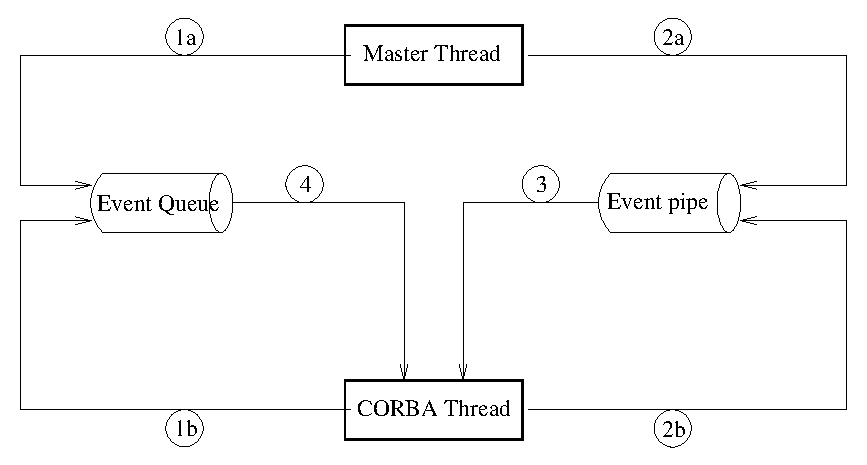
\includegraphics[width=\textwidth]{eventflow.eps}
\caption{\label{f_prog_event}Flow of control and data for event handling}
\end{figure}

\begin{enumerate}
\item The event itself is pushed into the master's event queue (defined in
line 85 in the \master\ header file). This can be done by either the
master thread (case a, responding to a \codapi\ request), or by the 
corba thread (case b, responding to a \qidl\ request).
This is the real \texttt{Codine::event} struct that is actually sent across
the network to the event channel.
Of course, the appropriate locks for the event queue must be obtained 
and released correctly.
\item A byte is written into the ORBacus event handler's pipe. The interesting
thing here is, that the \master\ singleton object itself is the event
handler that is addressed by this event.
\item The ORBacus Reactor, i.e. the event dispatching facility picks up the
event from the pipe and calls the event handling function, in this case
\texttt{Codine\_Master\_impl::handleEvent()}. Note that between steps 2 and
3, there is either a thread context switch (case a), or the \qidl\ request
that caused the event in the first place is served completely and has its
answer returned (case b). Only then will \texttt{handleEvent()} be invoked.
\item The \texttt{handleEvent()} function retrieves the event from the event
queue and
\item sends it to the event channel.
\end{enumerate}

Steps 1 and 2 are done in a function called \texttt{addEvent()}, declared in
line 57 and implemented as follows:

\begin{Verbatim}[fontsize=\small, frame=single]
void Codine_Master_impl::addEvent(const CORBA_Any& any) {
   QENTER("Master::addEvent");

   // forget it if there is no event service
   if(CORBA_is_nil(es))
      return;

   PthreadLock foo(&events_lock);

   // push event into event queue
   events.push(any);

   // notify that there is an event
   char x = 'x';
   write(obEventFd[1], &x, sizeof(char));
}
\end{Verbatim}

This code can be executed both on behalf of the master thread or the corba
thread. There are only a few places where the \texttt{addEvent()} method is
called from: to signal the creation and deletion of an object in one of the
functions declared in lines 53-56, or to signal the modification of an object
in the corresponding object's \texttt{changed()} function. 

\paragraph{Miscellaneous}
One last feature of the \master\ implementation class is the
\texttt{getMasterContext()} method. This returns a CORBA context that
authenticates the user as \texttt{root} on the local machine. This is of
course only used internally, when the \qidl\ server calls an IDL function
locally. Since it must supply a valid \texttt{cod\_auth} context with each of
these operations, there is a need for a central facility to provide it with
one. That's exactly what \texttt{getMasterContext()} is.

\subsubsection{\label{s_prog_server_objects}Fine-Tuning the Data Objects}
The \idlgen\ code generator produced pretty much of an object implementation,
but still there are some things left to be done by a "real" programmer. He or
she must therefore derive another class (usually called \texttt{\_impl}) from
the \idlgen-produced \texttt{\_implementation} class that implements the
missing methods (many of them declared pure virtual in the base class).

These methods include proper creation/initialization and destruction/clean\-up.
These are trivial and need not be mentioned further here. A more interesting
function is \texttt{getSelf()}. This is called by any IDL method
implementation to get the object's cull representation. Remember that this is
either the global one stored in the master's object repository, or a local
one in case of a private, non-public object, depending on the value of the
object's \texttt{creation} variable. A typical \texttt{getSelf()}
implementation looks like the following:

\begin{Verbatim}[fontsize=\small, frame=single]
lListElem* Codine_Queue_impl::getSelf() {
   if(creation != 0)
      return self;

   // if newSelf is set, then use newSelf, because newSelf is
   // valid (if !NULL) and definitely newer than self
   if(newSelf)
      return self = newSelf;

   AUTO_LOCK_MASTER;

   lCondition* cp = lWhere("%T(%I==%s)", QU_Type, QU_qname,
                                                (const char*)key);
   self = lFindFirst(Master_Queue_List, cp);
   lFreeWhere(cp);
   return self;
}
\end{Verbatim}

The code should be easy to understand. The purpose of the \texttt{newSelf}
variable is more interesting and has something to do with event handling. If
an object is changed, an event must be generated. But due to details in the
\codine\ kernel code, at the time the event is packaged, the new object state
is not yet saved in the master's global storage. So the kernel code calls an
object's \texttt{changed()} function with the new object state as its
parameter (its new identity, so-to-speak).

\begin{Verbatim}[fontsize=\small, frame=single]
void Codine_Queue_impl::changed(lListElem* _newSelf) {
   QENTER("Queue::changed");

   AUTO_LOCK_MASTER;
   // set self variable for now
   self = newSelf = _newSelf;

   lastEvent = qidl_event_count;

   // build header
   Codine_event ev;
   ev.type = Codine_ev_mod;
   ev.obj  = COD_QUEUE_LIST;
   ev.name = CORBA_string_dup( (creation!=0)?
               lGetString(newSelf, QU_qname):(const char*)key);
   ev.id   = 0; // not needed for queue
   ev.ref  = this;
   ev.count= qidl_event_count;
   
   // get state
   Codine_contentSeq* cs = 
      get_content(Codine_Master_impl::instance()->getMasterContext());
   ev.changes = *cs;
   delete cs;

   CORBA_Any any;
   any <<= ev;

   Codine_Master_impl::instance()->addEvent(any);

   // now we're ourselves again :-(
   newSelf = 0;
}
\end{Verbatim}

The only reason for this \texttt{newSelf} artistic is that the
\texttt{changed()} function
calls \texttt{get\_content()}, which in turn calls other \texttt{get\_}
functions, as described in the previous section. Since all of these
\texttt{get\_} functions call \texttt{getSelf()}, they would return wrong,
i.e. old values. So someone has to tell \texttt{getSelf()} to return the new
identity of the object by setting the \texttt{newSelf} variable. An important
precondition that must never be violated is that this code is executed by
only one thread at a time. Otherwise two concurrent threads could overwrite
the \texttt{newSelf} variable and produce confusing results.

Now back to some easier business. As mentioned earlier, \idlgen\ cannot
produce code for attributes that reference other objects. This is because
\codine's cull lists are a bit inconsistent in this point and do not use a
common referencing pattern. So each implementation for such a function looks
a bit different, but the main goal is to produce a CORBA sequence or object
reference out of a cull list element or vice versa. For a queue's attached
complexes, this is accomplished as follows:

\begin{Verbatim}[fontsize=\small, frame=single]
Codine_ComplexSeq* Codine_Queue_impl::get_complex_list(
                                       CORBA_Context* ctx) {
   // usual function header...

   // now build the list of object refs
   lList* cpxl = lGetList(self, QU_complex_list);
   lListElem* lep;
   Codine_Complex_impl* c;

   Codine_ComplexSeq* cpx = new Codine_ComplexSeq();
   for_each_cpp(lep, cpxl) {
      c = Codine_Master_impl::instance()->getComplexImpl(
                                       lGetString(lep, CX_name));
      if(c)
         cpx->append(Codine_Complex_impl::_duplicate(c));
   }
   
   return cpx;
}

cod_ulong Codine_Queue_impl::set_complex_list(
                  const Codine_ComplexSeq& val, CORBA_Context* ctx) {
   // usual function header...

   // make api request
   lListPtr      lp;
   lListPtr      alp;
   lList*        ltp;
   lListElem*    ep;
   lListElem*    lep;
   lEnumeration* what;
   
   if(creation != 0)
      ep = self;
   else {
      lp = lCreateList("My Queue List", QU_Type);
      lAppendElem(lp, ep = lCopyElem(self));
   }

   ltp = lCreateList("cplx list", CX_Type);

   for(CORBA_ULong i=0; i<val.length(); i++) {
      lAppendElem(ltp, lep = lCreateElem(CX_Type));
      lSetString(lep, CX_name, val[i]->get_name(ctx));
      // we don't need the other fields for QU_complex_list
   }
   lSetList(ep, QU_complex_list, ltp);

   if(creation != 0)       // that's it for a local (= new) object
      return 0; 

   // otherwise send api request
   what = lWhat("%T(%I %I)", QU_Type, QU_qname, QU_complex_list);
   
   alp = cod_api(COD_QUEUE_LIST, COD_API_MOD, &lp, NULL, what);
   lFreeWhat(what);

   throwErrors(alp); 

   // this one is set during the cod_api call
   return lastEvent;
}
\end{Verbatim}

The functions look very similar to those for fundamental data types or
structs, but usually involve a mapping from the object's identifier (i.e.
name or id) to its CORBA object representation.

To finish up an object's implementation, there are only two functions left to
write: The \texttt{get\_identifier()}, and the \texttt{add()} methods.
\texttt{identifier} in this context is the name of the object's identifying
attribute, e.g. \texttt{qname} for queues or \texttt{job\_id} for jobs. The
\texttt{add()} (or \texttt{submit()} function for jobs) adds a non-public
object---i.e. one returned by \texttt{Master::newXXX()}---to the object
repository permanently. Again, a typical implementation is straightforward,
like this:

\begin{Verbatim}[fontsize=\small, frame=single]
void Codine_Queue_impl::add(CORBA_Context* ctx) {
   QENTER("Queue::add");

   // this Queue has been added already ?
   if(creation == 0)
      return;
   
   AUTO_LOCK_MASTER;

   qidl_authenticate(ctx);

   // make api request
   lListPtr      lp;
   lListPtr      alp;
   lEnumeration* what;
   
   lp = lCreateList("My Queue List", QU_Type);
   lAppendElem(lp, self); // This cares for automatic deletion of self

   what = lWhat("%T(ALL)", QU_Type);

   alp = cod_api(COD_QUEUE_LIST, COD_API_ADD, &lp, NULL, what);
   lFreeWhat(what);

   throwErrors(alp);

   // if we're here, everything worked fine and we can set
   // creation to 0, thus saying that we are a REAL queue
   creation = 0;
}
\end{Verbatim}

Of course, if \texttt{creation==0} nothing needs to be done since this is
already a globally visible object. Otherwise a \texttt{COD\_API\_ADD} is
issued. This also cares for automatic event creation and correct object
management in the master object.

\subsection{\label{s_prog_patterns}Design Patterns}
\qidl\ was written with some design patterns in mind. This produces code that
is easier to extend and makes use of proven programming paradigms. It
furthermore puts the code on a commonly accepted basis of working uses of
object-oriented techniques.

\subsubsection{Generation Gap}
This pattern was taken from \cite[pp. 85-101]{b_vlissides}. It addresses the
problem of automatically generated classes like those created by \idlgen. If a
programmer modified the created files by hand, for example to add some
functions to the class or modify the classes implementation, all of these
changes would be overwritten by a subsequent invocation of the code
generator. The solution is to derive yet another class from the one created
and add and override methods there.

Actually, this pattern appears twice in \qidl. The \texttt{\_impl}
classes are derived from the automatically generated \texttt{\_implementation}
classes, which in turn are derived from the automatically generated
\texttt{\_skel} classes. Figure \ref{f_prog_generation_gap} illustrates this
in a class diagram.

\begin{figure}
\begin{center}
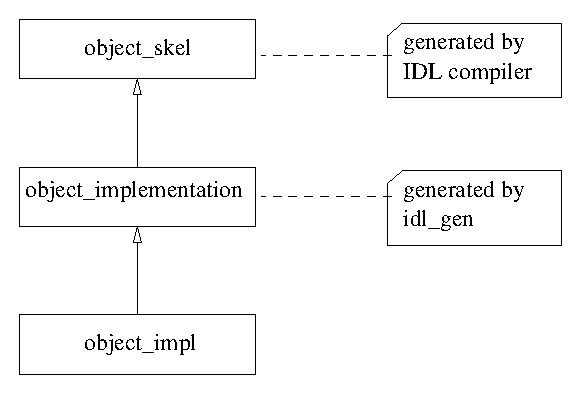
\includegraphics[height=3.8cm]{generationgap.eps}
\end{center}
\caption{\label{f_prog_generation_gap}Application of the \textsc{Generation
Gap} pattern in \qidl.}
\end{figure}

\subsubsection{\label{s_prog_singleton}Singleton and Abstract Factory}
Probably the most well-known and widely used design pattern is the
\textsc{Singleton} \cite[pp. 127-134]{b_gof}. It is used whenever there is
supposed to be only one instance of a class in one program. Singletons are
often used as an \textsc{Abstract Factory} \cite[pp. 87-95]{b_gof} as well.
These provide methods that create instances of other classes, but usually
return polymorphic subclasses.

The \texttt{Codine\_Master\_impl} class is such a combination of Singleton
and Abstract Factory. There is only one instance in the program (ensured by
the protected constructor and the \texttt{initialize()} function), and it
creates instances of other classes with its \texttt{newXXX()} methods, e.g.
\texttt{newJob()}. This is declared to return a \texttt{Codine\_Job} object,
but its implementation actually returns an object of type
\texttt{Codine\_Job\_impl}, which is 3 steps further down in the inheritance
hierarchy.

\subsubsection{Facade}
\textsc{Facade} \cite[pp. xx-yy]{b_gof} is a relatively unknown pattern. Its
purpose is to provide a simplified interface to clients that only need to
invoke one method of this interface. This in turn uses many correlated
objects in the background and possibly invokes several of their functions to
accomplish the desired task.

The \master\ interface provides a Facade to \qidl\ clients that want to
register and unregister a CORBA server that is running as a \codine\ job.
Without these functions, the client would have to retrieve the job list from
the master, find the appropriate job with its job id value and modify the
job's context attribute by appending the IOR to or deleting it from the
context list. Although not implemented yet, the \master\ object may provide
additional "shortcut" functions that perform complex, maybe even
transaction-like tasks with only one method invocation from the client.

\subsection{Tests}
\subsubsection{The Test Client}
To test the \qidl\ functionality, a simple and easily extensible test client
was developed. Its main program establishes a connection to the \qidl\
master as described in the user documentation, section
\ref{s_user_connecting}. It then evaluates the given command line arguments
and invokes a corresponding function via an array of function pointers. It is
defined as follows:

\begin{Verbatim}[fontsize=\small, frame=single]
typedef void (action_func)(Codine_Master_var master);
struct action {
   const char*   name;
   action_func*  func;
   const char*   desc;
   action(const char* n, action_func f, const char* d) :
            name(n), func(f), desc(d) {}
} actions[] = {
 action("simple", simple, "displays queues in an endless loop"),
 action("rw", readwrite, "reads and writes no. of slots of first q."),
 action("destroy", destroy, "prompts the user and destroys queues"),
 action("create", create, "prompts the user and creates a new queue"),
 action("qcplxmod", qcplxmod, "lets the user modify a q's complexes"),
 action("jobtest", jobtest, "displays jobs"),
 action("event", event, "acts as a simple event client"),
 action("doc_3", doc_sub, "the job submit example from the user doc")
};
\end{Verbatim}

Each entry in this array contains a name (the one that has to be specified in
the command line), the address of the corresponding function, and a short
description printed as a help message (shown when no argument is given). The
main program simply compares the command line argument with each of the names
from the array and calls the corresponding function to perform the desired
task. By adding a new function and an array entry, the test client can be
extended to test another feature of the \qidl\ server.

Several of these test clients, each of them running in an endless loop, in
addition to some conventional \codapi\ clients were run concurrently to
provoke race conditions and make load tests. Apart from producing serious
Linux/Alpha kernel crashes, they posed no problem to \qidl.

\subsubsection{JQmon}
Another important test facility was the Java version of Qmon. Its first
prototype was developed as part of a diploma thesis, using the C \codapi\ via
the Java Native Interface. This was replaced by CORBA by a Rumanian
guest student, Laurentiu Petrea, taking part in a European program.
JQmon was actually the first "real"
application to use \qidl, especially as an event client. This evaluated and
improved the event handling facility of \qidl, and---of course---surfaced
several bugs in the code.

\subsection{\label{s_prog_extending}Extending the Server}
This last section shows how easy it is to extend the \qidl\ server. The 
main ways of doing so is to

\begin{itemize}
\item add convenience functions
\item add new cull list elements to existing objects
\item add new objects
\end{itemize}

The first one is relatively easy. Just adding a method to the object's IDL
interface (between \texttt{/*IDL} and \texttt{XIDL*/}) in the api header
file, and implementing the function in the \texttt{\_impl} class is all there
is to do. Then it's only using the objects in a more or less intelligent way.

Adding new list elements is even easier if it is only a fundamental data type
or a struct---simply recompile \qidl! If the new element references another
object, you'll only have to write the \texttt{get\_} and \texttt{set\_}
methods. Usually, this is not very complicated as well.

Adding new objects like a queue or a job is a bit more work, although this
follows a common pattern applied to all other objects, too. There are several
steps to do.

\begin{enumerate}
\item Write the object's cull list in a (possibly new) api header file.
\item Append the object to the \texttt{OBJECTS} variable in the \qidl\
makefile. If it is in a new header file, don't forget to append the file to
the \texttt{IDLSRC} variable.
\item Write the object's implementation (see section
\ref{s_prog_server_objects}) in the \texttt{\_impl.h} and \texttt{\_impl.cpp}
files.
\item Extend the \master\ interface with the \texttt{getXXX()} and
\texttt{newXXX()} functions.
\item Extend the \texttt{Codine\_Master\_impl} class:
   \begin{enumerate}
   \item implement the new functions from the IDL interface.
   \item append a data member containing the list of object references.
   \item initialize the list in the \texttt{initialize()} method.
   \item provide the internal \texttt{getXXX()} and \texttt{getXXXImpl()}
   functions.
   \item extend the \texttt{addObject()} and \texttt{deleteObject()}
   functions to handle the new object type.
   \end{enumerate}
\item Write a new \texttt{object\_changed()} function in the 
\texttt{qidl\_c\_api} files and invoke this from somewhere in the \codine\ 
kernel code. This is usually done in the \texttt{cod\_add\_list\_event\_}
function.
\end{enumerate}
